

\section{Placa Indutivos}
\label{placa_01}


\begin{table}[ht!]

	\begin{tabular}{r l|l p{12cm} }
		
		\textcolor{gray}{Especificação} &&& 	{Placa Eletrônica Customizada}\\
		\textcolor{gray}{Data} &&& 				{03/12/2014}\\
        \textcolor{gray}{Beneficiado} &&&		{CIRVALE CIRCUITOS IMPRESSOS LTDA}
        \\
        \textcolor{gray}{CNPJ} &&& 				{23.292.279/0001-20} \\
        \textcolor{gray}{Número Nota} &&& 		{000.006.197} \\
		\textcolor{gray}{Quantidade} &&& 		{6} \\
		\textcolor{gray}{Valor} &&& 			{R\$352,44} \\
		\textcolor{gray}{Data Sheet} &&& 		{-} \\

		\textcolor{gray}{Função no projeto} &&& {A placa indutivo é responsável por
		alimentar e integrar os sensores indutivos, inclinação e pressão. A
		comunicação externa pode ser feita por RS485 ou Ethernet através de um
		conversor UART-Ethernet, o sch-remote.}
		\\
		\textcolor{gray}{Razão da Escolha} &&& {Empresa fornecedora do LEAD em
		diversos outros projetos. A qualidade do material e prazo de entrega sempre
		foi excelente.}

	\end{tabular}
\end{table}

\newpage
\subsection{Foto do Material}
\begin{figure}[H]
 \centering
 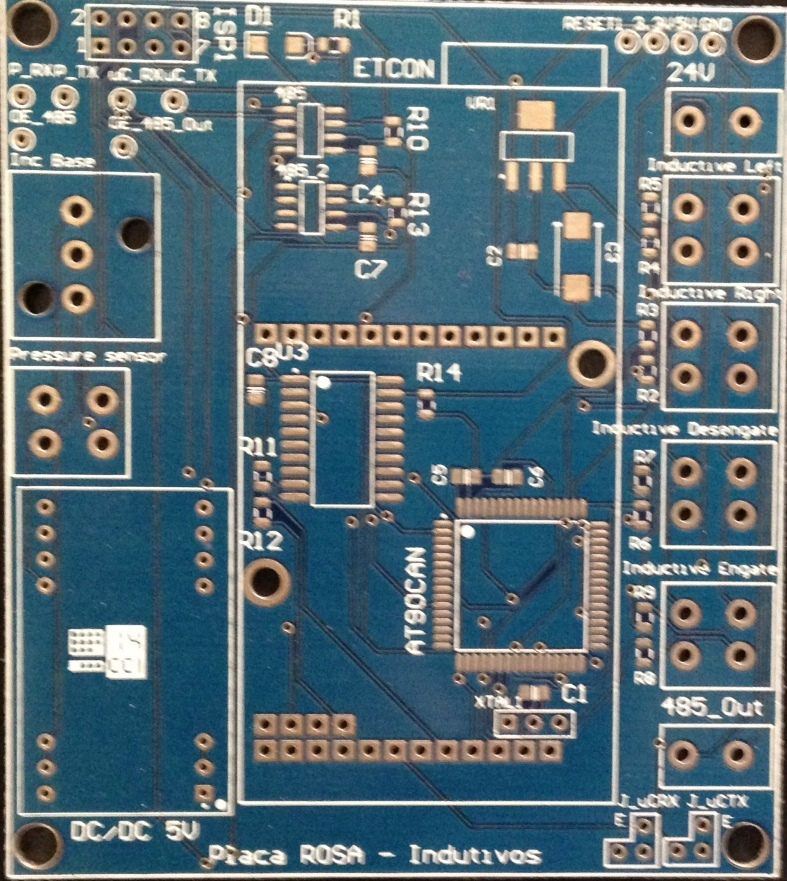
\includegraphics[width=0.5\columnwidth]{Placa/foto.jpg}
 \caption{Placa Indutivo}
\end{figure}

\subsection{Nota Fiscal}
\begin{figure}[H]
 \centering
 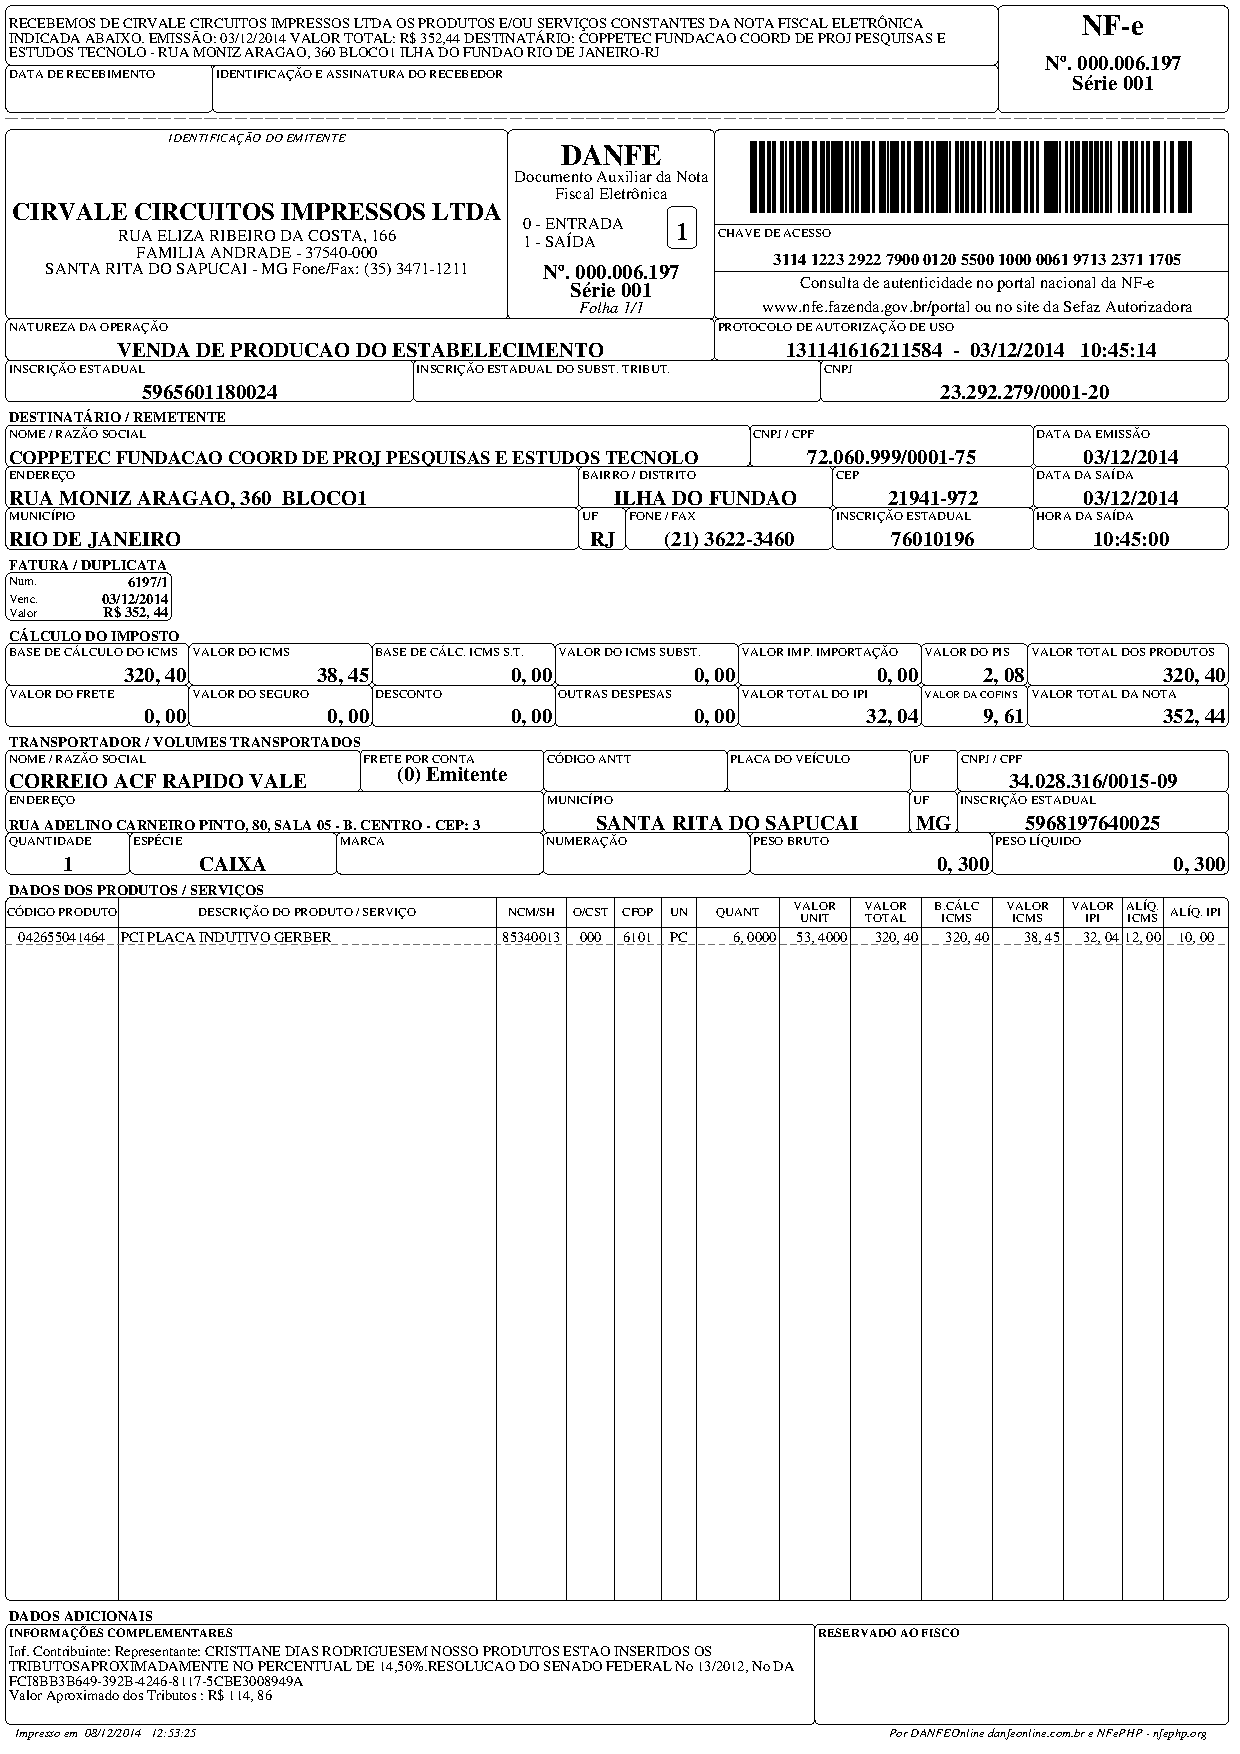
\includegraphics[width=0.9\columnwidth]{Placa/nota_placa.pdf}
 \caption{Placa Customizada Indutivos}
 \end{figure}